\uuid{ZvhB}
\exo7id{7082}
\titre{exo7 7082}
\auteur{megy}
\organisation{exo7}
\datecreate{2017-01-21}
\isIndication{false}
\isCorrection{true}
\chapitre{Géométrie affine euclidienne}
\sousChapitre{Géométrie affine euclidienne du plan}
\module{Géométrie}
\niveau{L2}
\difficulte{}

\contenu{
\texte{
% tags : symétrie centrale, réflexion orthogonale
Soit $ABC$ un triangle,  $P$ le pied de la hauteur issue de $A$ et $I$, $J$, $K$  les milieux des côtés $[AB]$, $[BC]$ et $[CA]$. Montrer que le quadrilatère $IPJK$ est un trapèze isocèle.
\begin{center}
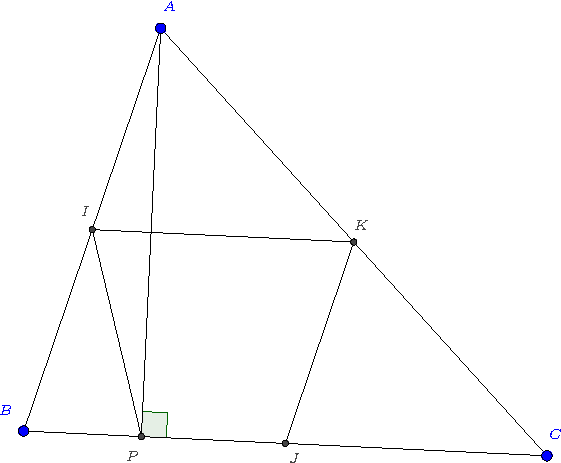
\includegraphics{../images/pdf/ZvhB-1.pdf}
\end{center}
}
}
